\clearpage
\section{Hardware}
\subsection{Raspberry PI}
The Raspberry PI is a small computer in the form of a single board with a system on a chip. The SoC is a BCM2835 licensed from Broadcom. It has an ARM11v6 CPU running at 700 MHz with 256 (model A) or 512 MB (model B) SDRAM shared with the on board GPU.
\begin{figure}[h]
    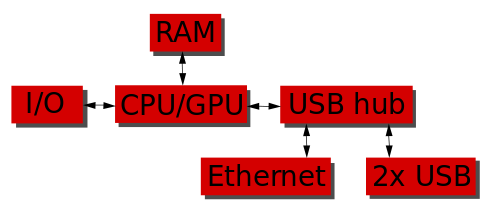
\includegraphics[width=0.5\textwidth]{hardware/raspberrypi_block_function}
    \caption{Layout of the functional blocks on the PI}
    \label{fig:pi_blockdiagram}
\end{figure}
\subsection{Configuration}
The PI comes with a number of different options for configuration. It can be overclocked and the memory split with the shared memory GPU can be set at boot using {\tt /boot/config.txt}.
Most unofficial documentation states that it requires a minimum of 16MB of RAM, but we were unable to get the PI to boot with less than 48 MB. With less than 48, it seems the system never gets to boot.
The setting on our running hardware is therefore {\tt gpu\_mem\_512=48}.

The Raspberry is also allows for easy overclocking without voiding the warranty, however reports suggest
\subsection{Alternative hardware}
\subsubsection{BeagleBone Black}
The BeagleBone Black is another open source low power mini pc on a single board. It is made by Texas Instruments and sold under the Creative Commons license.
The board is made from an AM3359 SoC from Texas Instruments, sporting an ARMv7 Cortex-A8 running at 1 GHz with 512MB of DDR3 RAM. This board has a slightly weaker GPU than the PI, which is of interest as we will not be using it anyway, and could help giving more power to the CPU.
We did not know about the release of this board when we did the planning for this project, but with it's very similar pricing (\$45 as of this writing) and significantly more powerful CPU, it would make for an interesting comparison and alternative. The reported power consumption is riddled with uncertainty, but reports seem to place it slightly higher to that of the PI, with 200-400 mA.
\subsubsection{MK802}

\subsection{Cluster}
\subsection{Power}
Our power supply is a 5V AC-DC converter with a maximum output of 4.2A at 5V. The expected maximum drain of the PI is listed at 700mA\cite{raspi_power_drain}. This would allow us to run at least $\frac{4.2A}{0.7A}=6$ PIs.
However we are not using the GPU or any other media related devices so we would expect this number to be somewhat lower, even under load.
